% !TEX program = pdflatex
\documentclass[aspectratio=169, 10pt]{beamer}

\usetheme{metropolis}

% ── Fonts (pdflatex-compatible) ───────────────────────────────────────
\usepackage[T1]{fontenc}
\usepackage{FiraSans}
\usepackage{FiraMono}

% ── Packages ──────────────────────────────────────────────────────────
\usepackage{tikz}
\usetikzlibrary{arrows.meta, positioning, calc, fit, backgrounds, shapes.geometric, decorations.pathreplacing, matrix}
\usepackage{booktabs}
\usepackage{tabularx}
\usepackage{listings}
\usepackage{multicol}
\usepackage{graphicx}
\usepackage{appendixnumberbeamer}
\usepackage{xcolor}
\usepackage{amsmath}

% ── Colours ───────────────────────────────────────────────────────────
\definecolor{peregrine}{HTML}{00B4D8}
\definecolor{accentgreen}{HTML}{06D6A0}
\definecolor{accentamber}{HTML}{FFD166}
\definecolor{accentred}{HTML}{EF476F}
\definecolor{codebg}{HTML}{1E1E2E}
\definecolor{layer0}{HTML}{5E548E}
\definecolor{layer1}{HTML}{2B6CB0}
\definecolor{layer2}{HTML}{2F855A}
\definecolor{layer3}{HTML}{C05621}
\definecolor{layer4}{HTML}{9B2C2C}
\definecolor{boxblue}{HTML}{1A365D}
\definecolor{boxgray}{HTML}{2D3748}

\setbeamercolor{progress bar}{fg=peregrine}
\setbeamercolor{alerted text}{fg=peregrine}

% ── Listings ──────────────────────────────────────────────────────────
\lstset{
  basicstyle=\ttfamily\tiny,
  keywordstyle=\color{peregrine}\bfseries,
  commentstyle=\color{gray},
  stringstyle=\color{accentgreen},
  backgroundcolor=\color{codebg},
  frame=single,
  rulecolor=\color{gray!30},
  breaklines=true,
  showstringspaces=false,
  tabsize=2,
  columns=fullflexible,
}

% ── TikZ styles ───────────────────────────────────────────────────────
\tikzset{
  mbox/.style={rectangle, rounded corners=3pt, draw=#1, fill=#1!15, thick,
               minimum height=0.7cm, text width=2.8cm, align=center,
               font=\scriptsize\bfseries},
  mbox/.default=peregrine,
  sbox/.style={rectangle, rounded corners=2pt, draw=#1, fill=#1!10, thick,
               minimum height=0.55cm, text width=2.2cm, align=center,
               font=\tiny\bfseries},
  sbox/.default=peregrine,
  lbl/.style={font=\tiny\itshape, text=gray},
  arr/.style={-{Stealth[length=4pt]}, thick, #1},
  arr/.default=gray,
  layerbox/.style={rectangle, rounded corners=4pt, draw=#1!70, fill=#1!8,
                   thick, minimum height=0.9cm, align=center, font=\scriptsize},
}

% ── Metadata ──────────────────────────────────────────────────────────
\title{PEREGRINE Flight Stack}
\subtitle{Architecture, Design \& Multi-Agent Integration}
\date{\today}
\author{}
\institute{}

% ══════════════════════════════════════════════════════════════════════
\begin{document}

% ── Title ─────────────────────────────────────────────────────────────
\maketitle

% ── Outline ───────────────────────────────────────────────────────────
\begin{frame}{Agenda}
\begin{columns}[T]
\begin{column}{0.48\textwidth}
\textbf{Part I --- Design \& Architecture}
\begin{enumerate}
  \item Project Overview \& Goals
  \item Layered Architecture
  \item Data Flow \& Timing
  \item Frame Convention Strategy
  \item Plugin Architecture
  \item Safety Architecture
  \item UAV Manager --- State Machine
\end{enumerate}
\end{column}
\begin{column}{0.48\textwidth}
\textbf{Part II --- Multi-Agent \& Deployment}
\begin{enumerate}\setcounter{enumi}{7}
  \item Multi-Agent Architecture
  \item Containerized Deployment
  \item Monitoring \& Visualization
\end{enumerate}
\vspace{0.5em}
\textbf{Part III --- Code Overview}
\begin{enumerate}\setcounter{enumi}{10}
  \item Interfaces \& Messages
  \item Key Package Walk-through
  \item Implementation Status
\end{enumerate}
\vspace{0.5em}
\textbf{Appendix} --- ROS\,2 \& PX4 Background
\end{column}
\end{columns}
\end{frame}


% ══════════════════════════════════════════════════════════════════════
\section{Part I: Design \& Architecture}
% ══════════════════════════════════════════════════════════════════════

% ── 1. Project Overview ──────────────────────────────────────────────
\begin{frame}{What is PEREGRINE?}
\textbf{PEREGRINE} --- \emph{Aerial Robotics Infrastructure for Operational Navigation}

A ROS\,2-based autonomous flight stack for \alert{multi-agent UAV operations} with PX4 autopilots.

\vspace{0.8em}
\begin{columns}[T]
\begin{column}{0.48\textwidth}
\textbf{Key Characteristics}
\begin{itemize}
  \item Manager-based modular architecture
  \item Plugin-based algorithms (swap at runtime)
  \item Multi-platform: simulation, Jetson Orin, RPi\,5
  \item Multi-agent with collision avoidance
  \item Safety-first with layered monitoring
  \item Fully containerized (Docker)
\end{itemize}
\end{column}
\begin{column}{0.48\textwidth}
\textbf{Technology Stack}
\begin{tabular}{@{}ll@{}}
\toprule
\scriptsize Language & \scriptsize C++17 \\
\scriptsize Middleware & \scriptsize ROS\,2 Humble / Jazzy \\
\scriptsize Autopilot & \scriptsize PX4 v1.15+ (uXRCE-DDS) \\
\scriptsize Simulation & \scriptsize Gazebo Harmonic, PX4 SITL \\
\scriptsize Math & \scriptsize Eigen\,3 \\
\scriptsize Plugins & \scriptsize ROS\,2 pluginlib \\
\scriptsize Containers & \scriptsize Docker + Compose \\
\scriptsize Inter-container & \scriptsize Zenoh bridge \\
\bottomrule
\end{tabular}
\end{column}
\end{columns}
\end{frame}

% ── Design Goals ─────────────────────────────────────────────────────
\begin{frame}{Design Goals}
\begin{tabularx}{\textwidth}{@{}lX@{}}
\toprule
\textbf{Goal} & \textbf{Approach} \\
\midrule
Modularity & Each functional domain is a separate ROS\,2 package with clean interfaces \\
Extensibility & Plugin architecture --- add new algorithms without modifying core \\
Safety & Three-layer safety: manager checks, safety monitor, PX4 hardware failsafes \\
Multi-agent & Namespace isolation, Buffered Voronoi Cell collision avoidance \\
Deployability & Docker images per platform, systemd for hardware deployment \\
Research-friendly & Swap controllers / estimators at runtime via service calls \\
\bottomrule
\end{tabularx}
\end{frame}

% ── 2. Layered Architecture ─────────────────────────────────────────
\begin{frame}{Layered Architecture}
\centering
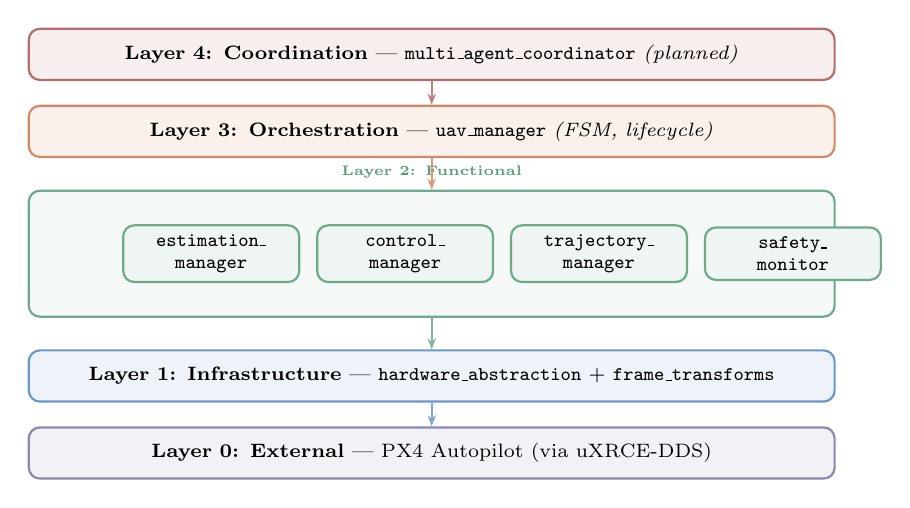
\begin{tikzpicture}[node distance=0.3cm, every node/.style={font=\scriptsize}]

  % Layer 4
  \node[layerbox=layer4, text width=10cm, minimum height=0.65cm]
    (l4) {\textbf{Layer 4: Coordination} --- \texttt{multi\_agent\_coordinator} \emph{(planned)}};

  % Layer 3
  \node[layerbox=layer3, text width=10cm, minimum height=0.65cm, below=of l4]
    (l3) {\textbf{Layer 3: Orchestration} --- \texttt{uav\_manager} \emph{(FSM, lifecycle)}};

  % Layer 2 — box in box
  \node[rectangle, rounded corners=4pt, draw=layer2!70, fill=layer2!5, thick,
        text width=10cm, minimum height=1.6cm, below=0.4cm of l3] (l2outer) {};
  \node[above=0.02cm of l2outer.north, anchor=south, font=\tiny\bfseries, text=layer2!80]
    {Layer 2: Functional};

  % Inner boxes inside L2
  \node[layerbox=layer2, minimum height=0.6cm, text width=2.0cm] (est) at ([xshift=-2.8cm]l2outer.center) {\texttt{estimation\_\\manager}};
  \node[layerbox=layer2, minimum height=0.6cm, text width=2.0cm, right=0.2cm of est] (ctrl) {\texttt{control\_\\manager}};
  \node[layerbox=layer2, minimum height=0.6cm, text width=2.0cm, right=0.2cm of ctrl] (traj) {\texttt{trajectory\_\\manager}};
  \node[layerbox=layer2, minimum height=0.6cm, text width=2.0cm, right=0.2cm of traj] (safe) {\texttt{safety\_\\monitor}};

  % Layer 1
  \node[layerbox=layer1, text width=10cm, minimum height=0.65cm, below=0.4cm of l2outer]
    (l1) {\textbf{Layer 1: Infrastructure} --- \texttt{hardware\_abstraction} + \texttt{frame\_transforms}};

  % Layer 0
  \node[layerbox=layer0, text width=10cm, minimum height=0.65cm, below=of l1]
    (l0) {\textbf{Layer 0: External} --- PX4 Autopilot (via uXRCE-DDS)};

  % Arrows
  \draw[arr=layer4!60] (l4) -- (l3);
  \draw[arr=layer3!60] (l3) -- (l2outer.north);
  \draw[arr=layer2!60] (l2outer.south) -- (l1);
  \draw[arr=layer1!60] (l1) -- (l0);
\end{tikzpicture}
\end{frame}

% ── Package Map ──────────────────────────────────────────────────────
\begin{frame}{Package Map}
\small
\begin{tabularx}{\textwidth}{@{}llcX@{}}
\toprule
\textbf{Package} & \textbf{Type} & \textbf{Layer} & \textbf{Purpose} \\
\midrule
\texttt{peregrine\_interfaces} & Interfaces & Cross & All custom msgs, srvs, actions \\
\texttt{frame\_transforms} & Library & 1 & ENU/NED conversions, TF2 broadcasting \\
\texttt{hardware\_abstraction} & Node & 1 & Sole PX4 interface, frame conversion boundary \\
\texttt{estimation\_manager} & Node + Plugins & 2 & State estimation plugin management \\
\texttt{control\_manager} & Node + Plugins & 2 & Flight controller plugin management \\
\texttt{trajectory\_manager} & Node + Plugins & 2 & Trajectory generation and evaluation \\
\texttt{safety\_monitor} & Node & 2 & Geofence, heartbeats, envelope protection \\
\texttt{uav\_manager} & Node & 3 & FSM, lifecycle, takeoff/land sequences \\
\texttt{tui\_status} & Node & Tool & ncurses real-time monitoring display \\
\texttt{peregrine\_bringup} & Launch/Config & Deploy & Launch files, YAML configs \\
\bottomrule
\end{tabularx}
\end{frame}

% ── 3. Data Flow ─────────────────────────────────────────────────────
\begin{frame}{Data Flow --- Control Loop}
\centering
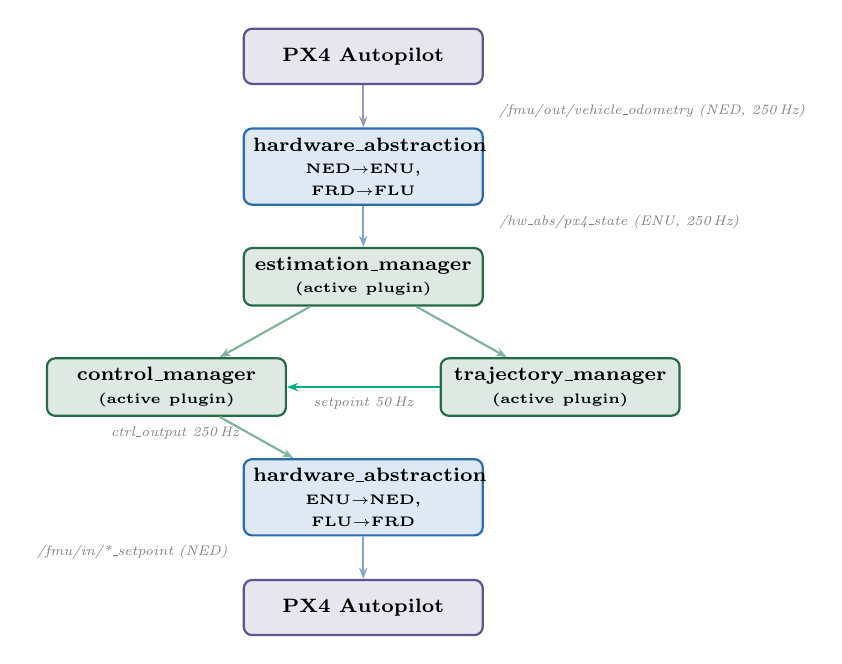
\begin{tikzpicture}[every node/.style={font=\scriptsize}]
  % Absolute positions to avoid off-screen issues
  \node[mbox=layer0] (px4t) at (0, 0) {PX4 Autopilot};
  \node[mbox=layer1] (hw1) at (0, -1.4) {hardware\_abstraction\\{\tiny NED$\to$ENU, FRD$\to$FLU}};
  \node[mbox=layer2!80!black] (est) at (0, -2.8) {estimation\_manager\\{\tiny (active plugin)}};
  \node[mbox=layer2!80!black] (ctrl) at (-2.5, -4.2) {control\_manager\\{\tiny (active plugin)}};
  \node[mbox=layer2!80!black] (traj) at (2.5, -4.2) {trajectory\_manager\\{\tiny (active plugin)}};
  \node[mbox=layer1] (hw2) at (0, -5.6) {hardware\_abstraction\\{\tiny ENU$\to$NED, FLU$\to$FRD}};
  \node[mbox=layer0] (px4b) at (0, -7.0) {PX4 Autopilot};

  % Labels
  \node[lbl, right] at (1.6, -0.7) {/fmu/out/vehicle\_odometry (NED, 250\,Hz)};
  \node[lbl, right] at (1.6, -2.1) {/hw\_abs/px4\_state (ENU, 250\,Hz)};
  \node[lbl, left] at (-1.6, -6.3) {/fmu/in/*\_setpoint (NED)};

  % Arrows
  \draw[arr=layer0!60] (px4t) -- (hw1);
  \draw[arr=layer1!60] (hw1) -- (est);
  \draw[arr=layer2!60] (est) -- (ctrl);
  \draw[arr=layer2!60] (est) -- (traj);
  \draw[arr=accentgreen!80!black, thick] (traj) -- node[lbl, below, pos=0.5] {setpoint 50\,Hz} (ctrl);
  \draw[arr=layer2!60] (ctrl) -- node[lbl, left, pos=0.4] {ctrl\_output 250\,Hz} (hw2);
  \draw[arr=layer1!60] (hw2) -- (px4b);
\end{tikzpicture}
\end{frame}

% ── Timing Requirements ──────────────────────────────────────────────
\begin{frame}{Timing Requirements}
\begin{tabularx}{\textwidth}{@{}lccp{5.5cm}@{}}
\toprule
\textbf{Loop} & \textbf{Frequency} & \textbf{Deadline} & \textbf{Notes} \\
\midrule
State estimation & 250\,Hz & 4\,ms & Matched to PX4 odometry rate \\
Control output & 250\,Hz & 4\,ms & Must be deterministic \\
Trajectory evaluation & 50\,Hz & 20\,ms & Setpoints interpolated at controller rate \\
Safety monitoring & 100\,Hz & 10\,ms & Highest priority --- independent watchdog \\
Offboard heartbeat & $\ge$\,2\,Hz & 500\,ms & PX4 requirement --- exits offboard if missed \\
TUI display & 10\,Hz & 100\,ms & Non-critical \\
\bottomrule
\end{tabularx}
\end{frame}

% ── 4. Frame Convention ──────────────────────────────────────────────
\begin{frame}{Frame Convention Strategy}
\begin{columns}[T]
\begin{column}{0.55\textwidth}
\textbf{The Problem:} PX4 uses NED/FRD, ROS\,2 uses ENU/FLU.\\
Mixing them is the \#1 source of ``drone flew the wrong way'' bugs.

\vspace{0.5em}
\textbf{Golden Rule:} All PEREGRINE packages operate in \alert{ENU/FLU}.\\
Conversion happens at \emph{exactly one point}: \texttt{hardware\_abstraction}.

\vspace{0.8em}
\centering
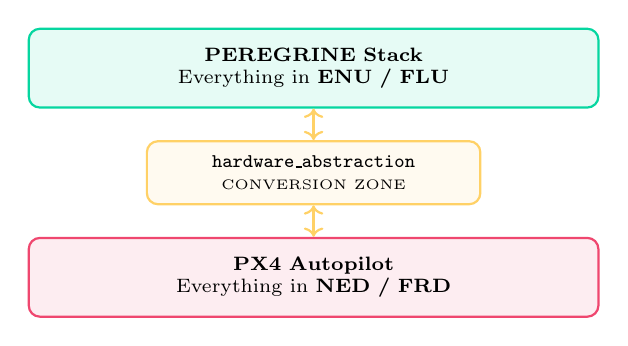
\begin{tikzpicture}[every node/.style={font=\scriptsize}]
  \node[rectangle, rounded corners=4pt, draw=accentgreen, fill=accentgreen!10, thick,
        text width=7cm, minimum height=1cm, align=center]
    (stack) {\textbf{PEREGRINE Stack}\\Everything in \textbf{ENU / FLU}};
  \node[rectangle, rounded corners=4pt, draw=accentamber, fill=accentamber!10, thick,
        text width=4cm, minimum height=0.8cm, align=center, below=0.4cm of stack]
    (hw) {\texttt{hardware\_abstraction}\\{\tiny CONVERSION ZONE}};
  \node[rectangle, rounded corners=4pt, draw=accentred, fill=accentred!10, thick,
        text width=7cm, minimum height=1cm, align=center, below=0.4cm of hw]
    (px4) {\textbf{PX4 Autopilot}\\Everything in \textbf{NED / FRD}};
  \draw[arr=accentamber, <->] (stack) -- (hw);
  \draw[arr=accentamber, <->] (hw) -- (px4);
\end{tikzpicture}
\end{column}

\begin{column}{0.42\textwidth}
\textbf{Conversion Summary}

\vspace{0.3em}
\scriptsize
\begin{tabular}{@{}lll@{}}
\toprule
\textbf{Qty} & \textbf{ENU$\to$NED} & \textbf{FLU$\to$FRD} \\
\midrule
Position & $(y, x, -z)$ & $(x, -y, -z)$ \\
Quaternion & $(w, y, x, -z)$ & same \\
Yaw & $\frac{\pi}{2} - \psi_{\text{enu}}$ & N/A \\
Covariance & $R\,C\,R^T$ & same \\
\bottomrule
\end{tabular}

\vspace{0.8em}
\normalsize
\textbf{TF2 Frame Tree} {\scriptsize(REP\,105/103)}

\vspace{0.3em}
\scriptsize
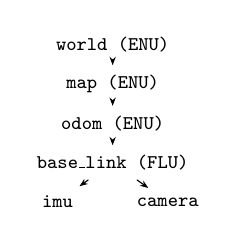
\begin{tikzpicture}[
  every node/.style={font=\scriptsize\ttfamily},
  level distance=0.5cm, sibling distance=1.4cm,
  edge from parent/.style={draw, -{Stealth[length=3pt]}, thin}
]
\node {world (ENU)}
  child { node {map (ENU)}
    child { node {odom (ENU)}
      child { node {base\_link (FLU)}
        child { node {imu} }
        child { node {camera} }
      }
    }
  };
\end{tikzpicture}
\end{column}
\end{columns}
\end{frame}

% ── 5. Plugin Architecture ───────────────────────────────────────────
\begin{frame}{Plugin Architecture}
\begin{columns}[T]
\begin{column}{0.52\textwidth}
\textbf{Design Rationale}

\vspace{0.3em}
\small
\begin{tabularx}{\columnwidth}{@{}lXX@{}}
\toprule
 & \textbf{Without} & \textbf{With Plugins} \\
\midrule
\scriptsize New algo & \scriptsize Modify core, recompile & \scriptsize Compile plugin, load via YAML \\
\scriptsize Runtime switch & \scriptsize Impossible & \scriptsize Service call \\
\scriptsize Testing & \scriptsize Full system & \scriptsize Mock interface \\
\bottomrule
\end{tabularx}

\vspace{0.6em}
\textbf{Plugin Lifecycle} (common to all managers)
\begin{enumerate}\small
  \item \texttt{initialize(node, name)} --- receive parent node
  \item \texttt{activate()} --- start processing
  \item \texttt{deactivate()} --- stop processing
  \item \texttt{reset()} --- clear internal state
\end{enumerate}
\end{column}

\begin{column}{0.45\textwidth}
\centering
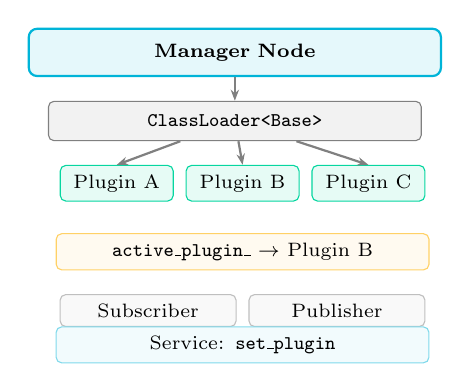
\begin{tikzpicture}[every node/.style={font=\scriptsize}, node distance=0.3cm]
  \node[rectangle, rounded corners=3pt, draw=peregrine, fill=peregrine!10, thick,
        text width=5cm, minimum height=0.6cm, align=center] (mgr) {\textbf{Manager Node}};

  \node[rectangle, rounded corners=2pt, draw=gray, fill=gray!10,
        text width=4.5cm, minimum height=0.5cm, align=center, below=0.3cm of mgr]
    (loader) {\texttt{ClassLoader<Base>}};

  \node[rectangle, rounded corners=2pt, draw=accentgreen, fill=accentgreen!10,
        text width=1.2cm, minimum height=0.4cm, align=center, below=0.3cm of loader, xshift=-1.5cm]
    (pa) {Plugin A};
  \node[rectangle, rounded corners=2pt, draw=accentgreen, fill=accentgreen!10,
        text width=1.2cm, minimum height=0.4cm, align=center, right=0.15cm of pa]
    (pb) {Plugin B};
  \node[rectangle, rounded corners=2pt, draw=accentgreen, fill=accentgreen!10,
        text width=1.2cm, minimum height=0.4cm, align=center, right=0.15cm of pb]
    (pc) {Plugin C};

  \node[rectangle, rounded corners=2pt, draw=accentamber, fill=accentamber!10,
        text width=4.5cm, minimum height=0.4cm, align=center, below=0.4cm of pb]
    (active) {\texttt{active\_plugin\_} $\to$ Plugin B};

  \node[rectangle, rounded corners=2pt, draw=gray!50, fill=gray!5,
        text width=2cm, minimum height=0.35cm, align=center, below=0.3cm of active, xshift=-1.2cm]
    (sub) {Subscriber};
  \node[rectangle, rounded corners=2pt, draw=gray!50, fill=gray!5,
        text width=2cm, minimum height=0.35cm, align=center, right=0.15cm of sub]
    (pub) {Publisher};
  \node[rectangle, rounded corners=2pt, draw=peregrine!50, fill=peregrine!5,
        text width=4.5cm, minimum height=0.35cm, align=center, below=0.2cm of $(sub)!0.5!(pub)$]
    (srv) {Service: \texttt{set\_plugin}};

  \draw[arr=gray] (loader) -- (pa.north);
  \draw[arr=gray] (loader) -- (pb.north);
  \draw[arr=gray] (loader) -- (pc.north);
  \draw[arr=gray] (mgr) -- (loader);
\end{tikzpicture}
\end{column}
\end{columns}
\end{frame}

% ── Three Plugin Domains ─────────────────────────────────────────────
\begin{frame}{Three Plugin Domains}
\small
\begin{tabularx}{\textwidth}{@{}llXXX@{}}
\toprule
\textbf{Domain} & \textbf{Base Class} & \textbf{Input} & \textbf{Output} & \textbf{Plugins} \\
\midrule
Estimation & \texttt{EstimatorBase} & PX4 state, ext.\ pose & \texttt{State} & PX4 Passthrough \\
\addlinespace
Control & \texttt{ControllerBase} & State + Setpoint & \texttt{ControlOutput} & PX4 Passthrough, SE(3) \\
\addlinespace
Trajectory & \texttt{TrajGeneratorBase} & Waypoints / goals & \texttt{TrajSetpoint} & Waypoint, Hold, Takeoff/Land \\
\bottomrule
\end{tabularx}

\vspace{0.8em}
\textbf{Control Hierarchy --- Where PEREGRINE Meets PX4}

\vspace{0.3em}
\centering
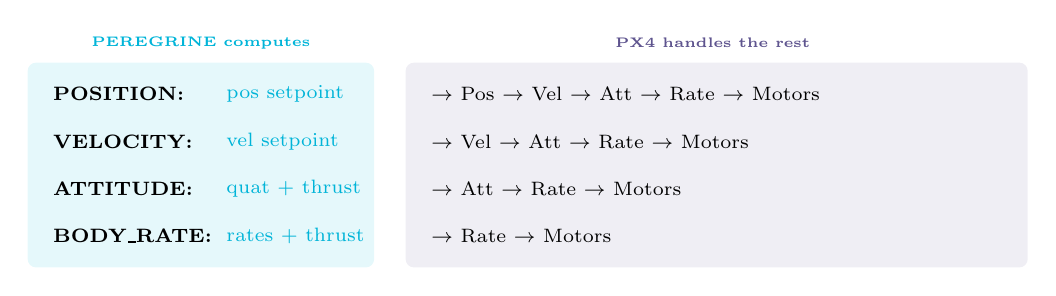
\begin{tikzpicture}[every node/.style={font=\scriptsize}, node distance=0.05cm]
  \fill[peregrine!10, rounded corners=3pt] (-0.2, 0) rectangle (4.2, 2.6);
  \fill[layer0!10, rounded corners=3pt] (4.6, 0) rectangle (12.5, 2.6);
  \node[font=\tiny\bfseries, peregrine] at (2, 2.85) {PEREGRINE computes};
  \node[font=\tiny\bfseries, layer0] at (8.5, 2.85) {PX4 handles the rest};

  \node[anchor=west] at (0, 2.2) {\textbf{POSITION:}};
  \node[anchor=west, peregrine] at (2.2, 2.2) {pos setpoint};
  \node[anchor=west] at (4.8, 2.2) {$\to$ Pos $\to$ Vel $\to$ Att $\to$ Rate $\to$ Motors};

  \node[anchor=west] at (0, 1.6) {\textbf{VELOCITY:}};
  \node[anchor=west, peregrine] at (2.2, 1.6) {vel setpoint};
  \node[anchor=west] at (4.8, 1.6) {$\to$ Vel $\to$ Att $\to$ Rate $\to$ Motors};

  \node[anchor=west] at (0, 1.0) {\textbf{ATTITUDE:}};
  \node[anchor=west, peregrine] at (2.2, 1.0) {quat + thrust};
  \node[anchor=west] at (4.8, 1.0) {$\to$ Att $\to$ Rate $\to$ Motors};

  \node[anchor=west] at (0, 0.4) {\textbf{BODY\_RATE:}};
  \node[anchor=west, peregrine] at (2.2, 0.4) {rates + thrust};
  \node[anchor=west] at (4.8, 0.4) {$\to$ Rate $\to$ Motors};
\end{tikzpicture}

\vspace{0.3em}
\small Lower modes $=$ more control authority for PEREGRINE; higher modes $=$ simpler companion code.
\end{frame}

% ── 6. Safety Architecture ───────────────────────────────────────────
\begin{frame}{Safety Architecture --- Three Layers}
\begin{columns}[T]
\begin{column}{0.55\textwidth}
\centering
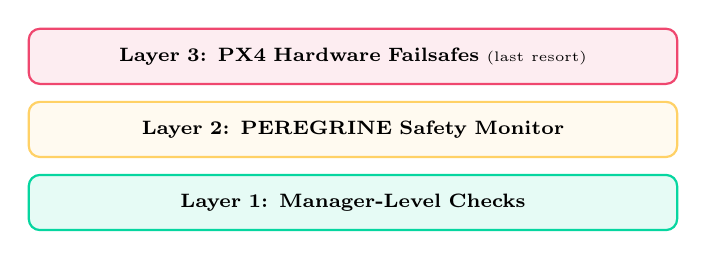
\begin{tikzpicture}[every node/.style={font=\scriptsize}, node distance=0.2cm]
  \node[rectangle, rounded corners=4pt, draw=accentred, fill=accentred!10, thick,
        text width=8cm, minimum height=0.7cm, align=center]
    (l3) {\textbf{Layer 3: PX4 Hardware Failsafes} {\tiny(last resort)}};

  \node[rectangle, rounded corners=4pt, draw=accentamber, fill=accentamber!10, thick,
        text width=8cm, minimum height=0.7cm, align=center, below=of l3]
    (l2) {\textbf{Layer 2: PEREGRINE Safety Monitor}};

  \node[rectangle, rounded corners=4pt, draw=accentgreen, fill=accentgreen!10, thick,
        text width=8cm, minimum height=0.7cm, align=center, below=of l2]
    (l1) {\textbf{Layer 1: Manager-Level Checks}};
\end{tikzpicture}

\vspace{0.4em}
\textbf{Safety Status State Machine}

\vspace{0.15em}
\centering
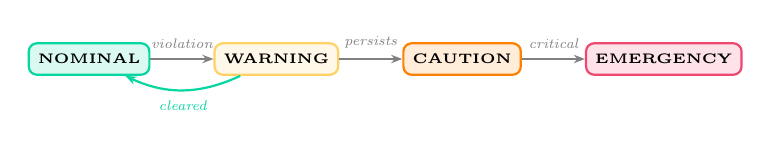
\begin{tikzpicture}[every node/.style={font=\tiny\bfseries}, node distance=0.8cm,
  state/.style={rectangle, rounded corners=3pt, draw, thick, minimum height=0.4cm, minimum width=1.1cm, align=center}]
  \node[state, draw=accentgreen, fill=accentgreen!15] (nom) {NOMINAL};
  \node[state, draw=accentamber, fill=accentamber!15, right=of nom] (warn) {WARNING};
  \node[state, draw=orange, fill=orange!15, right=of warn] (caut) {CAUTION};
  \node[state, draw=accentred, fill=accentred!15, right=of caut] (emer) {EMERGENCY};

  \draw[arr=gray] (nom) -- node[above, font=\tiny\itshape] {violation} (warn);
  \draw[arr=gray] (warn) -- node[above, font=\tiny\itshape] {persists} (caut);
  \draw[arr=gray] (caut) -- node[above, font=\tiny\itshape] {critical} (emer);
  \draw[arr=accentgreen, bend left=25] (warn) to node[below, font=\tiny\itshape] {cleared} (nom);
\end{tikzpicture}
\end{column}

\begin{column}{0.42\textwidth}
\textbf{Safety Checks}

\vspace{0.2em}
\tiny
\begin{tabular}{@{}lll@{}}
\toprule
\textbf{Check} & \textbf{Rate} & \textbf{Action} \\
\midrule
Geofence & 100\,Hz & Land/RTH \\
Heartbeat & Cont. & E-land/RTH \\
State valid. & 100\,Hz & Hover$\to$Land \\
Envelope & 100\,Hz & Limit output \\
Battery & 10\,Hz & Warn$\to$RTH$\to$Land \\
Collision & 20\,Hz & Slow$\to$Stop \\
\bottomrule
\end{tabular}

\vspace{0.3em}
\normalsize
\textbf{Heartbeat Priorities}

\vspace{0.2em}
\tiny
\begin{tabular}{@{}llll@{}}
\toprule
\textbf{Source} & \textbf{Priority} & \textbf{Timeout} & \textbf{Loss} \\
\midrule
hw\_abstraction & Critical & 1.0\,s & E-land \\
estimator\_mgr & Critical & 0.5\,s & E-land \\
control\_mgr & High & 0.5\,s & RTH \\
GCS & High & 5.0\,s & RTH \\
trajectory\_mgr & Medium & 1.0\,s & Hold \\
\bottomrule
\end{tabular}
\end{column}
\end{columns}
\end{frame}

% ── 7. UAV Manager State Machine ─────────────────────────────────────
\begin{frame}{UAV Manager --- State Machine}
\centering
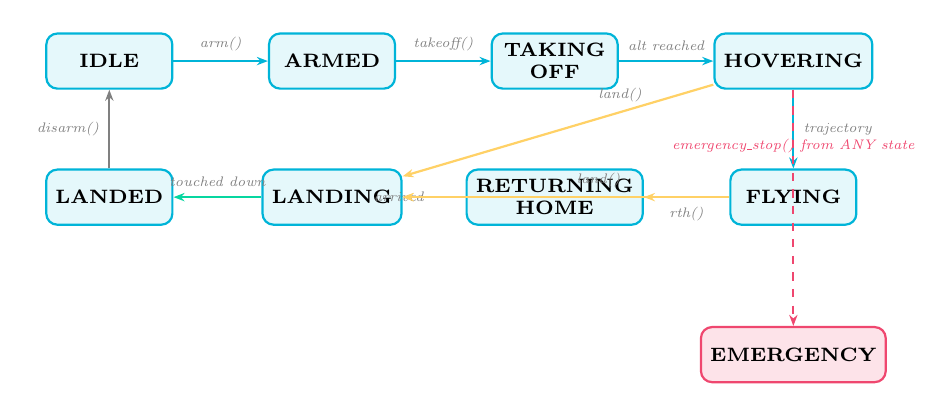
\begin{tikzpicture}[
  every node/.style={font=\scriptsize\bfseries},
  state/.style={rectangle, rounded corners=4pt, draw=peregrine, fill=peregrine!10,
                thick, minimum height=0.7cm, minimum width=1.6cm, align=center},
  emergency/.style={rectangle, rounded corners=4pt, draw=accentred, fill=accentred!15,
                    thick, minimum height=0.7cm, minimum width=1.6cm, align=center},
  node distance=0.6cm and 1.0cm
]
  \node[state] (idle) {IDLE};
  \node[state, right=1.2cm of idle] (armed) {ARMED};
  \node[state, right=1.2cm of armed] (takeoff) {TAKING\\OFF};
  \node[state, right=1.2cm of takeoff] (hover) {HOVERING};
  \node[state, below=1.0cm of hover] (fly) {FLYING};
  \node[state, below=1.0cm of takeoff] (rth) {RETURNING\\HOME};
  \node[state, below=1.0cm of armed] (land) {LANDING};
  \node[state, below=1.0cm of idle] (landed) {LANDED};
  \node[emergency, below=2.5cm of $(hover)!0.5!(fly)$] (emer) {EMERGENCY};

  \draw[arr=peregrine] (idle) -- node[above, font=\tiny\itshape, text=gray] {arm()} (armed);
  \draw[arr=peregrine] (armed) -- node[above, font=\tiny\itshape, text=gray] {takeoff()} (takeoff);
  \draw[arr=peregrine] (takeoff) -- node[above, font=\tiny\itshape, text=gray] {alt reached} (hover);
  \draw[arr=peregrine] (hover) -- node[right, font=\tiny\itshape, text=gray] {trajectory} (fly);
  \draw[arr=accentamber] (hover) -- node[above, font=\tiny\itshape, text=gray, pos=0.3] {land()} (land);
  \draw[arr=accentamber] (fly) -- node[below, font=\tiny\itshape, text=gray] {rth()} (rth);
  \draw[arr=accentamber] (rth) -- node[left, font=\tiny\itshape, text=gray] {arrived} (land);
  \draw[arr=accentamber] (fly.west) -- node[above, font=\tiny\itshape, text=gray, pos=0.4] {land()} (land.east);
  \draw[arr=accentgreen] (land) -- node[above, font=\tiny\itshape, text=gray] {touched down} (landed);
  \draw[arr=gray] (landed) -- node[left, font=\tiny\itshape, text=gray] {disarm()} (idle);

  % Emergency from any
  \draw[arr=accentred, dashed] (hover.south) -- ++(0,-0.5) -| node[pos=0.25, below, font=\tiny\itshape, text=accentred] {emergency\_stop() from ANY state} (emer.north);
\end{tikzpicture}
\end{frame}

% ── Preflight & Takeoff ──────────────────────────────────────────────
\begin{frame}{Preflight Checks \& Takeoff Sequence}
\begin{columns}[T]
\begin{column}{0.45\textwidth}
\textbf{Preflight Checks} (before arming)
\begin{enumerate}\small
  \item \texttt{hardware\_abstraction} connected to PX4
  \item \texttt{estimation\_manager} healthy \& publishing
  \item \texttt{control\_manager} has active controller
  \item \texttt{safety\_monitor} reports NOMINAL
  \item Battery above minimum threshold
  \item GPS fix adequate (outdoor) or MoCap (indoor)
  \item Geofence loaded and valid
\end{enumerate}
\end{column}

\begin{column}{0.50\textwidth}
\textbf{Takeoff Sequence}

\vspace{0.3em}
\small
\begin{enumerate}
  \item Assert state $=$ ARMED, run preflight checks
  \item Transition to TAKING\_OFF
  \item Request takeoff trajectory (target altitude)
  \item Command PX4 offboard mode
  \item \textbf{Loop:} publish feedback (altitude, progress\%)
    \begin{itemize}\scriptsize
      \item If safety alert or timeout $\to$ abort \& land
    \end{itemize}
  \item Altitude reached $\to$ transition to HOVERING
\end{enumerate}

\vspace{0.5em}
\textbf{Startup Order}

\vspace{0.2em}
\scriptsize
\texttt{hw\_abstraction} $\to$ \texttt{estimation\_mgr} $\to$ \texttt{control\_mgr} $\to$ \texttt{trajectory\_mgr} $\to$ \texttt{safety\_monitor} $\to$ \texttt{uav\_manager}
\end{column}
\end{columns}
\end{frame}

% ══════════════════════════════════════════════════════════════════════
\section{Part II: Multi-Agent \& Deployment}
% ══════════════════════════════════════════════════════════════════════

% ── 8. Multi-Agent Architecture ──────────────────────────────────────
\begin{frame}{Multi-Agent Architecture --- Overview}
\begin{columns}[T]
\begin{column}{0.45\textwidth}
\textbf{Implementation Status}

\vspace{0.3em}
\small
\begin{tabular}{@{}lc@{}}
\toprule
\textbf{Component} & \textbf{Status} \\
\midrule
Per-UAV namespace isolation & \alert{Done} \\
DDS domain container isolation & \alert{Done} \\
Zenoh inter-container bridging & \alert{Done} \\
Multi-instance PX4 SITL & \alert{Done} \\
GCS TUI multi-UAV view & \alert{Done} \\
BVC collision avoidance & Planned \\
Consensus protocols & Planned \\
Decentralized coordination & Planned \\
\bottomrule
\end{tabular}
\end{column}
\begin{column}{0.52\textwidth}
\textbf{Key Design Decisions}
\begin{itemize}\small
  \item \textbf{DDS domain isolation:} each UAV container has its own \texttt{ROS\_DOMAIN\_ID}
  \item \textbf{\texttt{ROS\_LOCALHOST\_ONLY=1}:} DDS stays within each container
  \item \textbf{Zenoh bridges:} selectively export only status topics (8 per UAV)
  \item \textbf{\texttt{network\_mode: host}:} all containers share host network for Zenoh
  \item \textbf{GCS domain 99:} isolated, receives only bridged status --- prevents accidental command injection
\end{itemize}
\end{column}
\end{columns}
\end{frame}

% ── Multi-Container Diagram ──────────────────────────────────────────
\begin{frame}{Multi-Container Architecture}
\centering
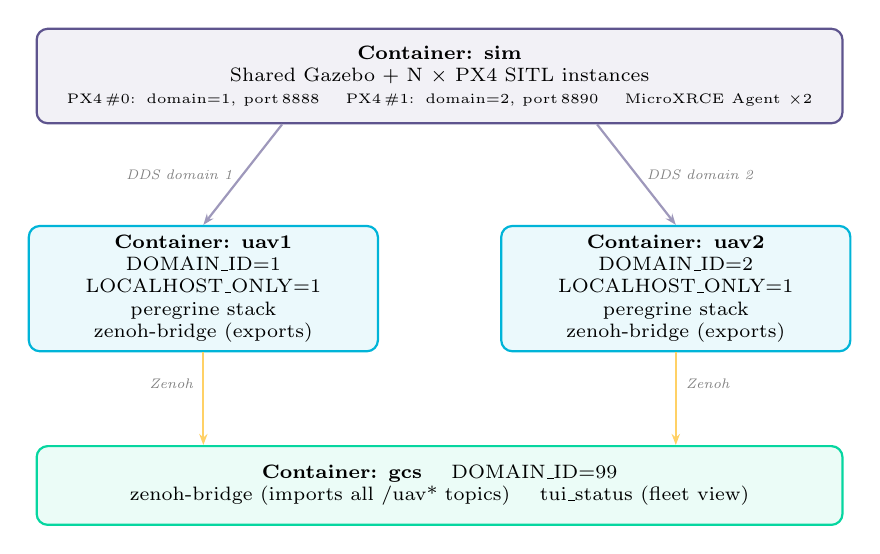
\begin{tikzpicture}[every node/.style={font=\scriptsize}]
  % Sim container — top center
  \node[rectangle, rounded corners=4pt, draw=layer0, fill=layer0!8, thick,
        text width=10cm, minimum height=1.2cm, align=center]
    (sim) at (0, 0) {\textbf{Container: sim}\\
            Shared Gazebo + N $\times$ PX4 SITL instances\\
            {\tiny PX4\,\#0: domain=1, port\,8888 \quad PX4\,\#1: domain=2, port\,8890 \quad MicroXRCE Agent $\times$2}};

  % UAV containers — side by side below sim
  \node[rectangle, rounded corners=4pt, draw=peregrine, fill=peregrine!8, thick,
        text width=4.2cm, minimum height=1.5cm, align=center]
    (uav1) at (-3, -2.7) {\textbf{Container: uav1}\\
             DOMAIN\_ID=1\\
             LOCALHOST\_ONLY=1\\
             peregrine stack\\
             zenoh-bridge (exports)};

  \node[rectangle, rounded corners=4pt, draw=peregrine, fill=peregrine!8, thick,
        text width=4.2cm, minimum height=1.5cm, align=center]
    (uav2) at (3, -2.7) {\textbf{Container: uav2}\\
             DOMAIN\_ID=2\\
             LOCALHOST\_ONLY=1\\
             peregrine stack\\
             zenoh-bridge (exports)};

  % GCS container — bottom center
  \node[rectangle, rounded corners=4pt, draw=accentgreen, fill=accentgreen!8, thick,
        text width=10cm, minimum height=1cm, align=center]
    (gcs) at (0, -5.2) {\textbf{Container: gcs} \quad DOMAIN\_ID=99\\
            zenoh-bridge (imports all /uav* topics) \quad tui\_status (fleet view)};

  % Arrows
  \draw[arr=layer0!60, thick] (sim.south) +(-2,0) -- node[left, lbl] {DDS domain 1} (uav1.north);
  \draw[arr=layer0!60, thick] (sim.south) +(2,0) -- node[right, lbl] {DDS domain 2} (uav2.north);
  \draw[arr=accentamber, thick] (uav1.south) -- node[left, lbl] {Zenoh} ++(0,-0.8) -| (gcs.north -| uav1);
  \draw[arr=accentamber, thick] (uav2.south) -- node[right, lbl] {Zenoh} ++(0,-0.8) -| (gcs.north -| uav2);
\end{tikzpicture}
\end{frame}

% ── Zenoh Bridge ─────────────────────────────────────────────────────
\begin{frame}{Zenoh Bridge --- Selective Topic Export}
\begin{columns}[T]
\begin{column}{0.45\textwidth}
\textbf{Bridged Topics per UAV} (8 total)

\vspace{0.3em}
\small
\begin{enumerate}
  \item \texttt{uav\_state} --- raw PX4 state
  \item \texttt{estimated\_state} --- filtered state
  \item \texttt{safety\_status} --- safety monitor output
  \item \texttt{estimation\_status} --- estimator health
  \item \texttt{control\_status} --- controller health
  \item \texttt{trajectory\_status} --- trajectory progress
  \item \texttt{status} --- comprehensive UAV status
  \item \texttt{gps\_status} --- GPS fix quality
\end{enumerate}
\end{column}
\begin{column}{0.50\textwidth}
\textbf{Why Zenoh?}
\begin{itemize}\small
  \item \texttt{ROS\_LOCALHOST\_ONLY} prevents DDS cross-container leaks
  \item Zenoh provides \emph{selective, explicit} topic sharing
  \item Status-only bridging: GCS observes but \emph{cannot inject commands}
  \item Peer-to-peer discovery --- no central broker needed
  \item Low-overhead protocol, works across networks
\end{itemize}

\vspace{0.5em}
\textbf{GCS Bridge}\\[0.2em]
\small
Subscribes to \texttt{uav*/} prefix and republishes on its local DDS domain (99).
\end{column}
\end{columns}
\end{frame}

% ── BVC Collision Avoidance ──────────────────────────────────────────
\begin{frame}{Planned: Buffered Voronoi Cell Collision Avoidance}
\begin{columns}[T]
\begin{column}{0.52\textwidth}
\textbf{Concept}\\[0.2em]
\small
Each UAV computes its own \emph{Voronoi cell} --- the region closer to itself than to any neighbor. The cell is shrunk inward by a safety buffer. If each UAV stays within its buffered cell, \alert{minimum separation is guaranteed}.

\vspace{0.5em}
\textbf{Algorithm} (per UAV $i$)\\[0.2em]
\small
For each neighbor $j$:
\begin{align*}
  \mathbf{m} &= \tfrac{1}{2}(\mathbf{p}_i + \mathbf{p}_j) \\
  \mathbf{n} &= \text{normalize}(\mathbf{p}_i - \mathbf{p}_j) \\
  \mathbf{b} &= \mathbf{m} + \mathbf{n} \cdot d_{\text{buffer}}
\end{align*}
\emph{Constraint:} $\mathbf{n} \cdot \mathbf{x} \le \mathbf{n} \cdot \mathbf{b}$

\vspace{0.3em}
Constraints published $\to$ \texttt{trajectory\_manager} projects setpoints onto feasible region.
\end{column}

\begin{column}{0.45\textwidth}
\centering
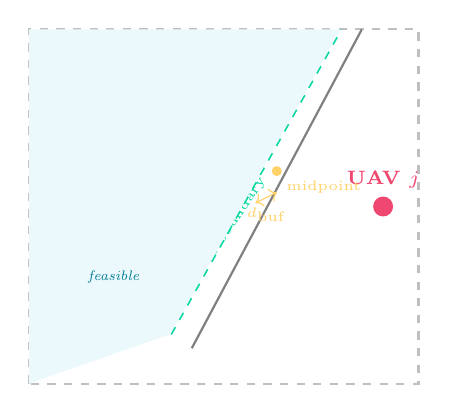
\begin{tikzpicture}[scale=0.9]
  % Voronoi-like regions
  \draw[thick, gray!50, dashed] (-2,-2) rectangle (3.5,3);

  % UAVs
  \fill[peregrine] (0, 1.5) circle (4pt) node[above=3pt, font=\scriptsize\bfseries] {UAV $i$};
  \fill[accentred] (3, 0.5) circle (4pt) node[above=3pt, font=\scriptsize\bfseries] {UAV $j$};

  % Midpoint
  \fill[accentamber] (1.5, 1.0) circle (2pt) node[below right, font=\tiny] {midpoint};

  % Voronoi boundary
  \draw[thick, gray] (0.3, -1.5) -- (2.7, 3.0);

  % Buffered boundary
  \draw[very thick, accentgreen, dashed] (0.0, -1.3) -- (2.4, 3.0);
  \node[font=\tiny, accentgreen, rotate=56] at (0.7, 0.0) {buffered boundary};

  % Buffer annotation
  \draw[<->, thin, accentamber] (1.2, 0.55) -- node[below, font=\tiny] {$d_{\text{buf}}$} (1.5, 0.7);

  % Feasible region shading
  \fill[peregrine!8] (-2,-2) -- (0.0,-1.3) -- (2.4,3.0) -- (-2,3.0) -- cycle;
  \node[font=\tiny\itshape, peregrine!70!black] at (-0.8, -0.5) {feasible};
\end{tikzpicture}
\end{column}
\end{columns}
\end{frame}

% ── 9. Docker & Deployment ───────────────────────────────────────────
\begin{frame}{Containerized Deployment}
\begin{columns}[T]
\begin{column}{0.48\textwidth}
\textbf{Docker Image Strategy}

\vspace{0.3em}
\small
\begin{tabular}{@{}llp{2.8cm}@{}}
\toprule
\textbf{Image} & \textbf{Platform} & \textbf{Features} \\
\midrule
\texttt{simulation} & x86 + NVIDIA & CUDA, Gazebo, PX4 SITL \\
\texttt{jetson} & arm64 & CUDA, TensorRT \\
\texttt{rpi5} & arm64 & Lightweight, headless \\
\bottomrule
\end{tabular}

\vspace{0.5em}
All images:
\begin{itemize}\scriptsize
  \item Mount full repo workspace $\to$ \texttt{/ros2\_ws}
  \item Non-root user mapped to host UID/GID
  \item \texttt{DRONE\_ID} $\to$ \texttt{ROS\_DOMAIN\_ID}
  \item Optionally start MicroXRCE Agent
\end{itemize}
\end{column}
\begin{column}{0.48\textwidth}
\textbf{Repository Structure}

\vspace{0.3em}
\ttfamily\scriptsize
\begin{tabbing}
\hspace{0.4cm}\=\hspace{0.4cm}\=\kill
peregrine/ \\
\> src/ \\
\>\> peregrine\_core/ {\normalfont\tiny(11 pkgs)} \\
\>\> px4\_msgs/ {\normalfont\tiny(submodule)} \\
\>\> peregrine\_app\_*/ {\normalfont\tiny(future)} \\
\> docker/ \\
\>\> docker/, compose/, config/ \\
\>\> Makefile \\
\> docs/
\end{tabbing}
\rmfamily

\vspace{0.5em}
\normalsize
\textbf{Operational Commands}
\scriptsize
\begin{tabular}{@{}ll@{}}
\texttt{make build-sim} & Build sim image \\
\texttt{make dev} & Dev shell (disposable) \\
\texttt{make multi-sitl} & 2-UAV sim + Zenoh \\
\texttt{DRONE\_ID=1 make jetson} & Run on Jetson \\
\end{tabular}
\end{column}
\end{columns}
\end{frame}

% ── 10. Monitoring ───────────────────────────────────────────────────
\begin{frame}{Monitoring --- TUI Status Display}
\begin{columns}[T]
\begin{column}{0.60\textwidth}
\centering
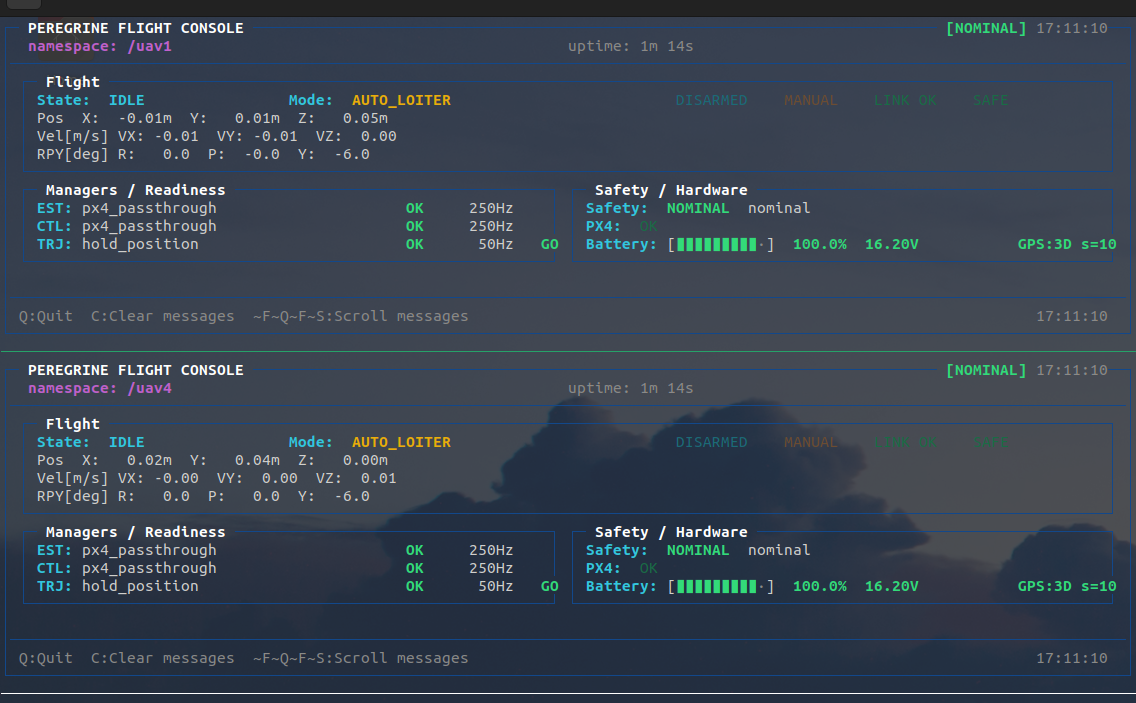
\includegraphics[width=\columnwidth]{debug_TUI.png}
\end{column}

\begin{column}{0.37\textwidth}
\textbf{ncurses Terminal UI}\\[0.2em]
Real-time monitoring at 10\,Hz

\vspace{0.4em}
\textbf{Features}
\begin{itemize}\scriptsize
  \item Color-coded: \textcolor{accentgreen}{green} (nominal), \textcolor{accentamber}{yellow} (warning), \textcolor{accentred}{red} (emergency)
  \item Multi-UAV compact fleet view
  \item Keyboard navigation between UAVs
  \item Alert ring buffer (100 entries)
  \item Non-blocking input
\end{itemize}

\vspace{0.4em}
\textbf{Display Sections}
\begin{itemize}\scriptsize
  \item Flight state, mode, armed status
  \item Position / velocity (ENU)
  \item Active manager plugins
  \item Safety status, geofence distance
  \item Connection health (heartbeats)
  \item Battery voltage / percent
\end{itemize}
\end{column}
\end{columns}
\end{frame}

% ── RViz Visualization ──────────────────────────────────────────────
\begin{frame}{Visualization --- RViz2 Multi-UAV}
\begin{columns}[T]
\begin{column}{0.60\textwidth}
\centering
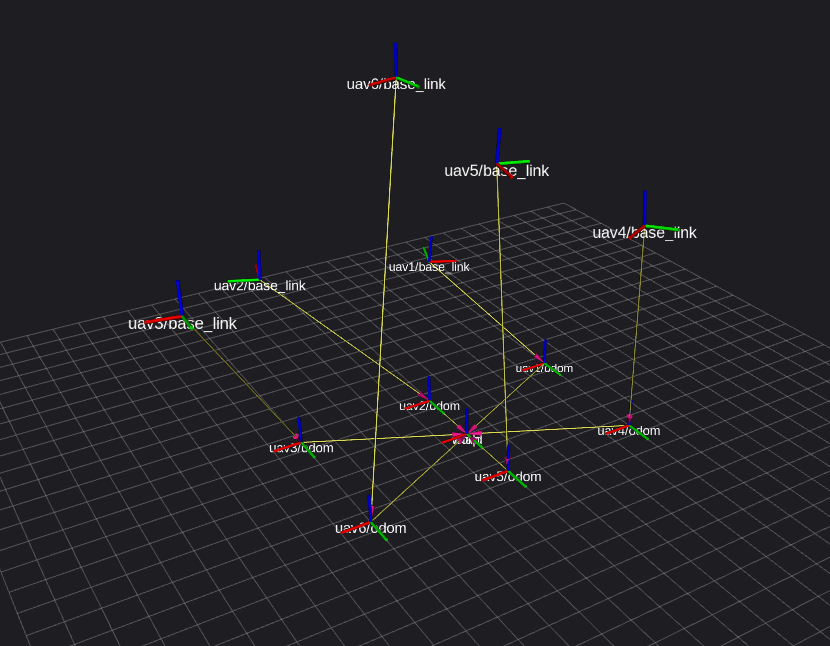
\includegraphics[width=\columnwidth]{6-uav_rviz.png}
\end{column}

\begin{column}{0.37\textwidth}
\textbf{RViz2 Flight Visualization}

\vspace{0.4em}
\begin{itemize}\small
  \item 6-UAV swarm visualization
  \item Per-UAV coordinate frames via TF2
  \item Real-time position and orientation
  \item Trajectory path display
  \item Multi-UAV markers with namespace isolation
  \item REP\,105 frame tree:\\
        {\scriptsize\texttt{world $\to$ map $\to$ odom $\to$ base\_link}}
\end{itemize}
\end{column}
\end{columns}
\end{frame}


% ══════════════════════════════════════════════════════════════════════
\section{Part III: Code Overview}
% ══════════════════════════════════════════════════════════════════════

% ── 11. Interfaces ───────────────────────────────────────────────────
\begin{frame}{Custom Interfaces --- \texttt{peregrine\_interfaces}}
\begin{columns}[T]
\begin{column}{0.48\textwidth}
\textbf{Design Principles}
\begin{itemize}\scriptsize
  \item \textbf{Single package} for all \texttt{.msg}, \texttt{.srv}, \texttt{.action}
  \item Semantic field names with units: \texttt{altitude\_m}, \texttt{velocity\_mps}
  \item Frame-explicit: all spatial msgs include \texttt{frame\_id}
  \item All messages timestamped via \texttt{std\_msgs/Header}
\end{itemize}

\vspace{0.3em}
\textbf{Core: State.msg}
\begin{itemize}\scriptsize
  \item Position (ENU), Velocity, Acceleration
  \item Orientation (quaternion ENU$\to$FLU)
  \item Angular velocity (FLU body) [rad/s]
  \item 6$\times$6 pose \& twist covariance
  \item Estimator name + confidence [0--1]
\end{itemize}

\vspace{0.3em}
\textbf{ControlOutput.msg}
\begin{itemize}\scriptsize
  \item \texttt{control\_mode}: POS / VEL / ATT / BODY\_RATE
  \item Mode-dependent fields; \texttt{thrust\_normalized} [0--1]
\end{itemize}
\end{column}

\begin{column}{0.48\textwidth}
\textbf{TrajectorySetpoint.msg}
\begin{itemize}\scriptsize
  \item Validity flags per field
  \item Position, velocity, acceleration, jerk, yaw, yaw\_rate
\end{itemize}

\vspace{0.2em}
\textbf{SafetyStatus.msg}
\begin{itemize}\scriptsize
  \item Safety level (NOMINAL $\to$ EMERGENCY)
  \item Component health flags, geofence status
  \item Heartbeat counts, battery, active alerts
  \item Recommended action
\end{itemize}

\vspace{0.2em}
\textbf{Actions}
\begin{itemize}\scriptsize
  \item Takeoff, Land, SetTrajectory, GoToPosition
\end{itemize}

\vspace{0.2em}
\textbf{Services}
\begin{itemize}\scriptsize
  \item SetController, SetEstimator, Arm, EmergencyStop
\end{itemize}
\end{column}
\end{columns}
\end{frame}

% ── 12. Key Packages ─────────────────────────────────────────────────
\begin{frame}{Hardware Abstraction --- Sole PX4 Interface}
\begin{columns}[T]
\begin{column}{0.50\textwidth}
\textbf{Bidirectional Translation}

\vspace{0.3em}
\centering
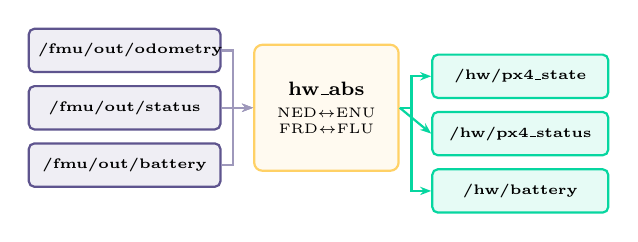
\begin{tikzpicture}[every node/.style={font=\tiny}, node distance=0.3cm]
  % FROM PX4
  \node[sbox=layer0, text width=2.2cm] (fmu_odom) {/fmu/out/odometry};
  \node[sbox=layer0, below=0.15cm of fmu_odom, text width=2.2cm] (fmu_stat) {/fmu/out/status};
  \node[sbox=layer0, below=0.15cm of fmu_stat, text width=2.2cm] (fmu_batt) {/fmu/out/battery};

  \node[rectangle, rounded corners=3pt, draw=accentamber, fill=accentamber!10, thick,
        text width=1.6cm, minimum height=1.6cm, align=center, right=0.4cm of fmu_stat]
    (hw) {\scriptsize\textbf{hw\_abs}\\[2pt]\tiny NED$\leftrightarrow$ENU\\FRD$\leftrightarrow$FLU};

  \node[sbox=accentgreen, right=0.4cm of hw, text width=2.0cm, yshift=0.4cm] (px4s) {/hw/px4\_state};
  \node[sbox=accentgreen, below=0.15cm of px4s, text width=2.0cm] (px4st) {/hw/px4\_status};
  \node[sbox=accentgreen, below=0.15cm of px4st, text width=2.0cm] (batt) {/hw/battery};

  \draw[arr=layer0!60] (fmu_odom.east) -- ++(0.15,0) |- (hw.west);
  \draw[arr=layer0!60] (fmu_stat.east) -- (hw.west);
  \draw[arr=layer0!60] (fmu_batt.east) -- ++(0.15,0) |- (hw.west);
  \draw[arr=accentgreen] (hw.east) -- ++(0.15,0) |- (px4s.west);
  \draw[arr=accentgreen] (hw.east) -- (px4st.west);
  \draw[arr=accentgreen] (hw.east) -- ++(0.15,0) |- (batt.west);
\end{tikzpicture}
\end{column}

\begin{column}{0.47\textwidth}
\textbf{Key Responsibilities}
\begin{itemize}\scriptsize
  \item Frame conversion at the boundary
  \item PX4 QoS matching (best-effort, transient-local)
  \item Offboard mode heartbeat ($\ge$\,2\,Hz)
  \item NaN convention for unused fields
  \item Time sync (PX4 $\mu$s $\leftrightarrow$ ROS\,2 ns)
  \item Arm/disarm service
  \item Control output $\to$ PX4 setpoint topic
\end{itemize}

\vspace{0.3em}
\textbf{Critical:} Wrong QoS = \emph{silent} comm failure. PX4 requires best-effort + transient-local.
\end{column}
\end{columns}
\end{frame}

% ── SE(3) Controller ─────────────────────────────────────────────────
\begin{frame}{SE(3) Geometric Controller}
\begin{columns}[T]
\begin{column}{0.55\textwidth}
\textbf{Geometric Tracking on SE(3)}\\
{\scriptsize\itshape Lee, Leok, McClamroch --- ``Geometric Tracking Control of a Quadrotor UAV on SE(3)''}

\vspace{0.5em}
\small
\textbf{Algorithm:}
\begin{enumerate}\small
  \item Position error: $\mathbf{e}_p = \mathbf{p} - \mathbf{p}_d$
  \item Velocity error: $\mathbf{e}_v = \mathbf{v} - \mathbf{v}_d$
  \item Desired accel: $\mathbf{a}_d = -K_p \mathbf{e}_p - K_d \mathbf{e}_v + \mathbf{a}_{ff} - g\,\hat{\mathbf{z}}$
  \item Desired thrust dir: $\hat{\mathbf{z}}_d = \text{normalize}(\mathbf{a}_d)$
  \item Thrust magnitude: $F = m\,(\mathbf{a}_d \cdot \hat{\mathbf{z}}_b)$
  \item Construct $R_d$ from $\hat{\mathbf{z}}_d$ + desired yaw
  \item \textbf{Output:} desired quaternion + normalized thrust
\end{enumerate}

\vspace{0.3em}
Output mode: \texttt{ATTITUDE} $\to$ PX4 attitude controller handles rate + motors
\end{column}

\begin{column}{0.42\textwidth}
\textbf{Configurable Gains}

\vspace{0.3em}
\small
\begin{tabular}{@{}ll@{}}
\toprule
\textbf{Parameter} & \textbf{Default} \\
\midrule
$K_p$ (position) & [6.0, 6.0, 8.0] \\
$K_d$ (velocity) & [4.5, 4.5, 5.0] \\
$K_{p,\text{att}}$ & [8.0, 8.0, 2.0] \\
$K_{d,\text{att}}$ & [1.5, 1.5, 0.4] \\
Mass & 1.5\,kg \\
Max thrust & 30.0\,N \\
\bottomrule
\end{tabular}

\vspace{0.5em}
\textbf{Adding a Custom Controller}
\begin{enumerate}\scriptsize
  \item Implement \texttt{ControllerBase}
  \item Register with \texttt{PLUGINLIB\_EXPORT\_CLASS}
  \item Add to config YAML
  \item Switch at runtime via service
\end{enumerate}
\end{column}
\end{columns}
\end{frame}

% ── Trajectory Manager ───────────────────────────────────────────────
\begin{frame}{Trajectory Manager}
\begin{columns}[T]
\begin{column}{0.50\textwidth}
\textbf{Available Generators}

\vspace{0.2em}
\scriptsize
\begin{tabular}{@{}llp{2.2cm}@{}}
\toprule
\textbf{Generator} & \textbf{Output} & \textbf{Use Case} \\
\midrule
WaypointLinear & POS+YAW & Linear interpolation \\
HoldPosition & POS+YAW & Hover, e-hold \\
TakeoffLand & POS+YAW & Vertical w/ S-curve \\
Polynomial & FULL & Min-snap (planned) \\
\bottomrule
\end{tabular}

\vspace{0.3em}
\small\textbf{Setpoint Loop} (50\,Hz)
\begin{enumerate}\scriptsize
  \item Compute elapsed $= t_{\text{now}} - t_{\text{start}}$
  \item Evaluate setpoint from generator
  \item Check BVC collision constraints
  \item If violating $\to$ project onto boundary
  \item Publish setpoint; mark completed when done
\end{enumerate}
\end{column}
\begin{column}{0.47\textwidth}
\textbf{Action Interface}

\vspace{0.2em}
\scriptsize
\textbf{SetTrajectory}: goal (trajectory + replace flag), feedback (progress \%, error), result (success/fail)

\vspace{0.2em}
\textbf{GoToPosition}: goal (target ENU, yaw, velocity), feedback (distance, ETA), result (success/fail)

\vspace{0.3em}
\small\textbf{Constraint Integration}\\[0.1em]
\scriptsize
BVC half-plane constraints from multi-agent coordinator are applied during setpoint evaluation. Violating setpoints are projected onto the nearest feasible point.
\end{column}
\end{columns}
\end{frame}

% ── 13. Implementation Status ────────────────────────────────────────
\begin{frame}{Implementation Status}
\small
\begin{tabularx}{\textwidth}{@{}lcX@{}}
\toprule
\textbf{Package} & \textbf{Status} & \textbf{Notes} \\
\midrule
\texttt{peregrine\_interfaces} & \textcolor{accentgreen}{Done} & All messages, services, actions defined \\
\texttt{frame\_transforms} & \textcolor{accentgreen}{Done} & Conversions + TF broadcaster, unit tested \\
\texttt{hardware\_abstraction} & \textcolor{accentgreen}{Done} & PX4 bridge, all control modes, time sync \\
\texttt{estimation\_manager} & \textcolor{accentgreen}{Done} & Manager + PX4 passthrough plugin \\
\texttt{control\_manager} & \textcolor{accentgreen}{Done} & Manager + PX4 passthrough + SE(3) geometric \\
\texttt{trajectory\_manager} & \textcolor{accentgreen}{Done} & Waypoint linear + hold + takeoff/land \\
\texttt{safety\_monitor} & \textcolor{accentgreen}{Done} & Geofence, battery, envelope, GPS, rule engine \\
\texttt{uav\_manager} & \textcolor{accentgreen}{Done} & State machine, preflight, takeoff/land \\
\texttt{tui\_status} & \textcolor{accentgreen}{Done} & Single + multi-UAV views, ncurses \\
\texttt{peregrine\_bringup} & \textcolor{accentgreen}{Done} & Launch files, configs, multi-UAV SITL \\
Docker stack + Zenoh & \textcolor{accentgreen}{Done} & Sim/Jetson/RPi5 images, inter-container bridging \\
\addlinespace
\texttt{multi\_agent\_coord.} & \textcolor{accentamber}{Planned} & BVC, consensus, decentralized coordination \\
Polynomial trajectories & \textcolor{accentamber}{Planned} & Minimum-snap trajectory generation \\
Custom EKF estimator & \textcolor{accentamber}{Planned} & Multi-sensor fusion \\
\bottomrule
\end{tabularx}
\end{frame}

% ── Summary ──────────────────────────────────────────────────────────
\begin{frame}{Summary}
\begin{columns}[T]
\begin{column}{0.48\textwidth}
\textbf{What PEREGRINE Provides}
\begin{itemize}
  \item Modular, plugin-based flight stack
  \item Clean PX4 integration with single conversion boundary
  \item Three-layer safety architecture
  \item Multi-agent support with container isolation + Zenoh
  \item Research-friendly: swap algorithms at runtime
  \item Multi-platform deployment (sim, Jetson, RPi5)
\end{itemize}
\end{column}
\begin{column}{0.48\textwidth}
\textbf{Next Steps}
\begin{itemize}
  \item BVC collision avoidance implementation
  \item Minimum-snap polynomial trajectories
  \item Custom EKF for multi-sensor fusion
  \item Decentralized coordination protocols
  \item Hardware flight testing campaign
  \item Distributed task allocation
\end{itemize}
\end{column}
\end{columns}

\vspace{1em}
\centering
\large\alert{Questions?}
\end{frame}


% ══════════════════════════════════════════════════════════════════════
\appendix
\section{Appendix: ROS\,2 \& PX4 Background}
% ══════════════════════════════════════════════════════════════════════

\begin{frame}{A.1 --- What is ROS\,2?}
\begin{itemize}
  \item Robot Operating System 2 --- middleware framework (not an OS)
  \item Built on DDS (Data Distribution Service) for real-time distributed communication
  \item Language support: C++, Python (PEREGRINE uses \textbf{C++17})
\end{itemize}

\vspace{0.5em}
\textbf{Core Communication Primitives}

\vspace{0.3em}
\begin{tabularx}{\textwidth}{@{}lllX@{}}
\toprule
\textbf{Primitive} & \textbf{Pattern} & \textbf{Blocking?} & \textbf{Use Case} \\
\midrule
Topics & Pub/Sub (many-to-many) & No & Sensor streams, state estimates, control outputs \\
Services & Request/Response (1:1) & Yes & Config changes, one-shot commands \\
Actions & Goal/Feedback/Result & No & Long-running: takeoff, trajectory execution \\
\bottomrule
\end{tabularx}
\end{frame}

\begin{frame}{A.2 --- ROS\,2 QoS \& Execution Model}
\begin{columns}[T]
\begin{column}{0.48\textwidth}
\textbf{Quality of Service (QoS)}

\vspace{0.3em}
\small
\begin{tabular}{@{}lll@{}}
\toprule
\textbf{Profile} & \textbf{Reliability} & \textbf{Use Case} \\
\midrule
Sensor Data & Best Effort & High-rate streams \\
Parameters & Reliable + TL & Config, late join \\
Default & Reliable & Services, actions \\
\bottomrule
\end{tabular}

\vspace{0.3em}
\begin{itemize}\scriptsize
  \item \textbf{Best Effort}: drop if subscriber can't keep up
  \item \textbf{Reliable}: retransmit until received
  \item \textbf{Transient Local}: late joiners get last value
  \item QoS mismatch $=$ \emph{silent} communication failure
\end{itemize}
\end{column}

\begin{column}{0.48\textwidth}
\textbf{Executors \& Callback Groups}
\begin{itemize}\small
  \item \textbf{Node}: smallest computation unit
  \item \textbf{Executor}: dispatches callbacks to threads
  \item \texttt{SingleThreaded}: one callback at a time
  \item \texttt{MultiThreaded}: concurrent (PEREGRINE uses this)
  \item \textbf{MutuallyExclusive} group: implicit mutex
  \item \textbf{Reentrant} group: user manages thread safety
\end{itemize}

\vspace{0.3em}
\textbf{Lifecycle (Managed) Nodes}
\begin{itemize}\scriptsize
  \item Unconfigured $\to$ Inactive $\to$ \textbf{Active} $\to$ Inactive
  \item Enables coordinated startup ordering
  \item PEREGRINE managers use lifecycle + \texttt{auto\_start}
\end{itemize}
\end{column}
\end{columns}
\end{frame}

\begin{frame}{A.3 --- ROS\,2 Namespaces \& pluginlib}
\begin{columns}[T]
\begin{column}{0.48\textwidth}
\textbf{Namespaces for Multi-Robot}

\vspace{0.3em}
\scriptsize
\begin{tabular}{@{}ll@{}}
\toprule
\textbf{Single UAV} & \textbf{Multi-UAV} \\
\midrule
\texttt{/hw\_abs/px4\_state} & \texttt{/uav1/hw\_abs/px4\_state} \\
\texttt{/est\_mgr/state} & \texttt{/uav1/est\_mgr/state} \\
& \texttt{/uav2/hw\_abs/px4\_state} \\
& \texttt{/uav2/est\_mgr/state} \\
\bottomrule
\end{tabular}

\vspace{0.3em}
\normalsize
\begin{itemize}\small
  \item ROS\,2 namespaces isolate per robot
  \item DDS Domain IDs for network-level isolation
  \item Combined with \texttt{LOCALHOST\_ONLY} for containers
\end{itemize}
\end{column}

\begin{column}{0.48\textwidth}
\textbf{pluginlib --- Runtime Plugin Loading}

\vspace{0.3em}
\begin{itemize}\small
  \item Load C++ classes at runtime from shared libraries
  \item Base class defines interface, plugins implement
  \item Registration: XML descriptors + \texttt{PLUGINLIB\_EXPORT\_CLASS}
  \item No recompilation of manager for new algorithms
\end{itemize}

\vspace{0.3em}
\textbf{Launch System}
\begin{itemize}\small
  \item Python-based launch files
  \item Supports arguments, conditionals, environment variables
  \item Include other launch files for modularity
\end{itemize}
\end{column}
\end{columns}
\end{frame}

\begin{frame}{A.4 --- PX4 Autopilot Overview}
\begin{columns}[T]
\begin{column}{0.50\textwidth}
\textbf{What is PX4?}
\begin{itemize}\scriptsize
  \item Open-source autopilot for drones, VTOL, rovers
  \item Low-level flight control: attitude stabilization, motor mixing, failsafes
  \item Runs on dedicated hardware (Pixhawk, etc.)
  \item PEREGRINE interfaces as companion computer stack
\end{itemize}

\vspace{0.2em}
\textbf{Offboard Mode}
\begin{itemize}\scriptsize
  \item PX4 accepts external commands from companion
  \item Must publish \texttt{OffboardControlMode} $\ge$\,2\,Hz
  \item Start publishing \emph{before} requesting mode switch
  \item Setpoint stream determines control level
\end{itemize}
\end{column}

\begin{column}{0.47\textwidth}
\textbf{PX4 Control Cascade}

\vspace{0.2em}
\centering
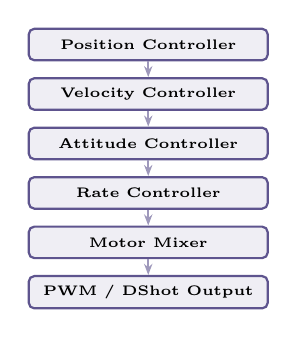
\begin{tikzpicture}[every node/.style={font=\tiny\bfseries},
  box/.style={rectangle, rounded corners=2pt, draw=layer0, fill=layer0!10,
              thick, minimum height=0.4cm, text width=2.8cm, align=center}]
  \node[box] (pos) {Position Controller};
  \node[box, below=0.2cm of pos] (vel) {Velocity Controller};
  \node[box, below=0.2cm of vel] (att) {Attitude Controller};
  \node[box, below=0.2cm of att] (rate) {Rate Controller};
  \node[box, below=0.2cm of rate] (mix) {Motor Mixer};
  \node[box, below=0.2cm of mix] (pwm) {PWM / DShot Output};

  \draw[arr=layer0!60] (pos) -- (vel);
  \draw[arr=layer0!60] (vel) -- (att);
  \draw[arr=layer0!60] (att) -- (rate);
  \draw[arr=layer0!60] (rate) -- (mix);
  \draw[arr=layer0!60] (mix) -- (pwm);
\end{tikzpicture}
\end{column}
\end{columns}
\end{frame}

\begin{frame}{A.5 --- uXRCE-DDS Bridge \& Frame Conventions}
\begin{columns}[T]
\begin{column}{0.45\textwidth}
\textbf{uXRCE-DDS Bridge}

\vspace{0.3em}
\centering
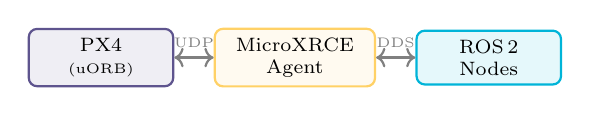
\begin{tikzpicture}[every node/.style={font=\scriptsize},
  box/.style={rectangle, rounded corners=3pt, draw, thick, minimum height=0.6cm, align=center}]
  \node[box, draw=layer0, fill=layer0!10, text width=1.6cm] (px4) {PX4\\{\tiny (uORB)}};
  \node[box, draw=accentamber, fill=accentamber!10, text width=1.8cm, right=0.5cm of px4]
    (agent) {MicroXRCE\\Agent};
  \node[box, draw=peregrine, fill=peregrine!10, text width=1.6cm, right=0.5cm of agent]
    (ros) {ROS\,2\\Nodes};

  \draw[arr=gray, <->] (px4) -- node[above, font=\tiny] {UDP} (agent);
  \draw[arr=gray, <->] (agent) -- node[above, font=\tiny] {DDS} (ros);
\end{tikzpicture}

\vspace{0.3em}
\begin{itemize}\scriptsize
  \item Replaces MAVLink for ROS\,2 integration
  \item PX4: \texttt{/fmu/out/*} (from), \texttt{/fmu/in/*} (to)
\end{itemize}

\vspace{0.3em}
\textbf{Key Points}
\begin{itemize}\scriptsize
  \item Frame mismatch = \#1 source of direction bugs
  \item PEREGRINE: all internal in ENU/FLU
  \item Single conversion in \texttt{hardware\_abstraction}
\end{itemize}
\end{column}

\begin{column}{0.52\textwidth}
\textbf{PX4 (NED/FRD) vs ROS\,2 (ENU/FLU)}

\vspace{0.2em}
\centering
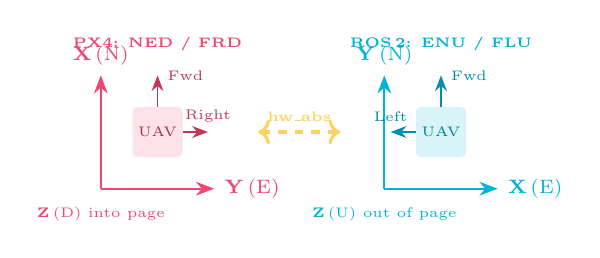
\begin{tikzpicture}[every node/.style={font=\scriptsize}, scale=0.8]
  % --- PX4 NED (left) ---
  \begin{scope}[shift={(0,0)}]
    \node[font=\tiny\bfseries, accentred, align=center] at (0.9, 2.3) {PX4: NED / FRD};
    % World: X=North(up), Y=East(right), Z=Down(into page)
    \draw[-{Stealth}, thick, accentred] (0,0) -- (0,1.8) node[above] {\textbf{X}\,(N)};
    \draw[-{Stealth}, thick, accentred] (0,0) -- (1.8,0) node[right] {\textbf{Y}\,(E)};
    \node[font=\tiny, accentred] at (0, -0.4) {\textbf{Z}\,(D) into page};
    % Body: top-view drone facing North
    \fill[accentred!15, rounded corners=2pt] (0.5, 0.5) rectangle (1.3, 1.3);
    \node[font=\tiny, accentred!70!black] at (0.9, 0.9) {UAV};
    \draw[-{Stealth}, semithick, accentred!80!black] (0.9,1.3) -- (0.9,1.8) node[right, font=\tiny] {Fwd};
    \draw[-{Stealth}, semithick, accentred!80!black] (1.3,0.9) -- (1.7,0.9) node[above, font=\tiny] {Right};
  \end{scope}

  % --- Conversion arrow ---
  \draw[<->, very thick, accentamber, dashed] (2.5, 0.9) -- node[above, font=\tiny\bfseries] {hw\_abs} (3.8, 0.9);

  % --- ROS2 ENU (right) ---
  \begin{scope}[shift={(4.5,0)}]
    \node[font=\tiny\bfseries, peregrine, align=center] at (0.9, 2.3) {ROS\,2: ENU / FLU};
    % World: X=East(right), Y=North(up), Z=Up(out of page)
    \draw[-{Stealth}, thick, peregrine] (0,0) -- (1.8,0) node[right] {\textbf{X}\,(E)};
    \draw[-{Stealth}, thick, peregrine] (0,0) -- (0,1.8) node[above] {\textbf{Y}\,(N)};
    \node[font=\tiny, peregrine] at (0, -0.4) {\textbf{Z}\,(U) out of page};
    % Body: top-view drone facing North (up in ENU = +Y)
    \fill[peregrine!15, rounded corners=2pt] (0.5, 0.5) rectangle (1.3, 1.3);
    \node[font=\tiny, peregrine!70!black] at (0.9, 0.9) {UAV};
    \draw[-{Stealth}, semithick, peregrine!80!black] (0.9,1.3) -- (0.9,1.8) node[right, font=\tiny] {Fwd};
    \draw[-{Stealth}, semithick, peregrine!80!black] (0.5,0.9) -- (0.1,0.9) node[above, font=\tiny] {Left};
  \end{scope}
\end{tikzpicture}

\vspace{0.2em}
\scriptsize
\begin{tabular}{@{}lll@{}}
\toprule
 & \textbf{World} & \textbf{Body} \\
\midrule
PX4 & NED: X$=$N, Y$=$E, Z$=$D & FRD: Fwd, Right, Down \\
ROS\,2 & ENU: X$=$E, Y$=$N, Z$=$U & FLU: Fwd, Left, Up \\
\bottomrule
\end{tabular}
\end{column}
\end{columns}
\end{frame}

\begin{frame}{A.6 --- PX4 SITL \& Configuration}
\begin{columns}[T]
\begin{column}{0.48\textwidth}
\textbf{PX4 Software-In-The-Loop}
\begin{itemize}\small
  \item Full PX4 autopilot on host machine
  \item Connects to Gazebo Harmonic for physics
  \item Identical code to what runs on hardware
  \item Multi-instance: N PX4 instances with different ports/domain IDs
\end{itemize}

\vspace{0.3em}
\textbf{PEREGRINE Config Structure}

\vspace{0.2em}
\ttfamily\scriptsize
\begin{tabbing}
\hspace{0.3cm}\=\hspace{0.3cm}\=\kill
config/ \\
\> default.yaml \\
\> environments/ \\
\>\> gps.yaml, mocap.yaml \\
\> uav\_types/ \\
\>\> quadrotor\_x.yaml \\
\> fleet/ \\
\>\> 4\_uav\_diamond.yaml
\end{tabbing}
\rmfamily
\end{column}

\begin{column}{0.48\textwidth}
\textbf{Key Default Parameters}

\vspace{0.3em}
\scriptsize
\begin{tabular}{@{}lll@{}}
\toprule
\textbf{Node} & \textbf{Parameter} & \textbf{Value} \\
\midrule
hw\_abstraction & offboard\_rate\_hz & 10.0 \\
estimator\_mgr & publish\_rate\_hz & 250.0 \\
 & default\_estimator & px4\_passthrough \\
control\_mgr & control\_rate\_hz & 250.0 \\
 & default\_controller & px4\_passthrough \\
trajectory\_mgr & publish\_rate\_hz & 50.0 \\
 & default\_generator & waypoint\_linear \\
uav\_manager & takeoff\_alt\_m & 2.0 \\
safety\_monitor & check\_rate\_hz & 100.0 \\
 & max\_radius\_m & 100.0 \\
 & max\_altitude\_m & 50.0 \\
\bottomrule
\end{tabular}

\vspace{0.5em}
\normalsize
\textbf{Launch Hierarchy}
\begin{itemize}\scriptsize
  \item \texttt{simulation.launch.py} $\to$ \texttt{single\_uav\_sitl} $\to$ \texttt{single\_uav}
  \item \texttt{multi\_uav\_sitl.launch.py} $\to$ N $\times$ UAV containers
\end{itemize}
\end{column}
\end{columns}
\end{frame}

\end{document}
